This version of fieldstone is a test of a instantaneous temperature equation solver.
This fieldstone is based on several benchmarks detailed earlier  in the manual, as well as a benchmark written by Tom Weir.
The T Weir benchmark (benchmark 0) is as follows:
\begin{eqnarray}
v_x &=& 0 \\
v_y &=& \frac{+2y-2y^3-6x^2y}/{-3x^2y^2+x^2}
T   &=& y x^2-y^3x^2
\end{eqnarray}
This benchmark has prescribed boundary conditions and has a domain of 0,1 in the y dimension and 0.75,1 in the x dimension.

The benchmark 1 is taken from section ??.[N.B. No label for initial_temperature.tex] It is based on simple conduction with no advection or heating. The domain is 0,1 and 0,1. The lower boundary has a prescribed temperature of $T=0$, and on the upper boundary $T=1$. This leads to a temperature profile given by $T=y$.

The benchmark 2 is, like the previous benchmark, based on section ??. It uses the same domain and boundary conditions, but features a constant heating term $H=1$. This leads to a temperature profile given by $T=\frac{3}{2}y-\frac{1}{2}y^2$.

The benchmark 3 is given in section \ref{mms6}, and is taken from \cite{ilpe07}. It is an convection-conduction benchmark, with the addition of a frictional heating/viscous dissapation term. The domain used is -1,+1 and -1,+1. The temperature is prescribed to be zero on both the upper and lower boundaries. THe velocity and temperature are as follows:
\begin{eqnarray}
v_x &=&  u_0(1-y**2) \\
v_y &=& 0 \\
T   &=& \frac{1}{3} \frac{\eta u_0^2}{k}
\end{eqnarray}
where $\eta$ is the viscosity and $k$ is the conductivity.
Two methods are used for the frictional heating. In the first, the analytical value is used in the solver. In the second, the strain rate is computed using the analytical velocity, and this strain rate is used to calculate the frictional heating in the solver. The former method is more accurate, as expected.

\begin{figure}
	\centering
	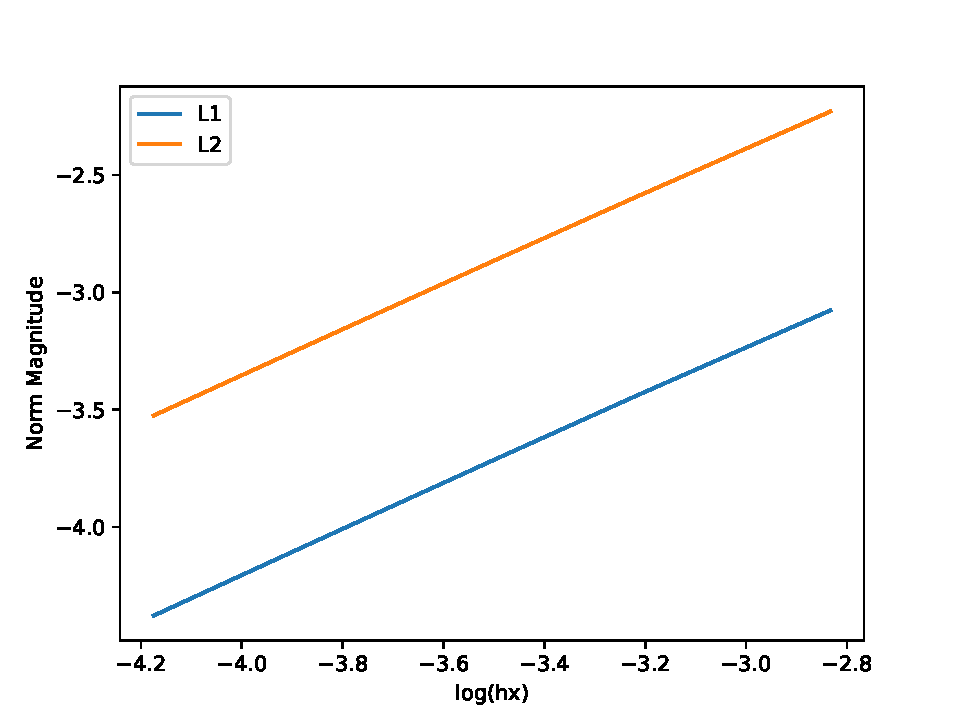
\includegraphics[width=0.8\textwidth]{temp_conv0.pdf}
	\caption{Convergence for benchmark 0}
\end{figure}

\begin{figure}
	\centering
	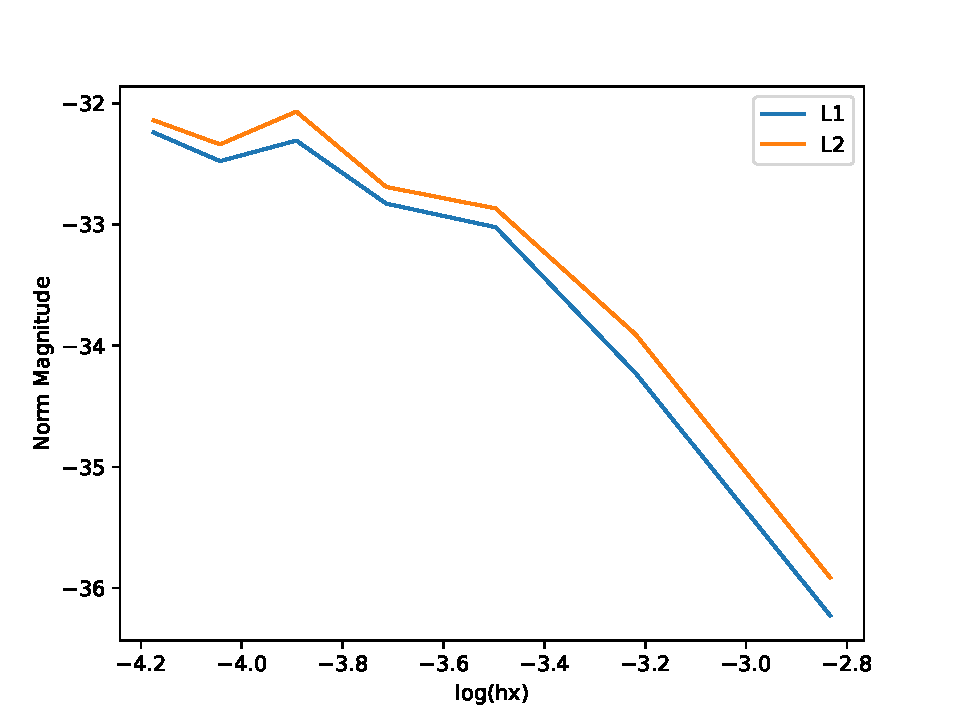
\includegraphics[width=0.8\textwidth]{temp_conv1.pdf}
	\caption{Convergence for benchmark 1}
\end{figure}

\begin{figure}
	\centering
	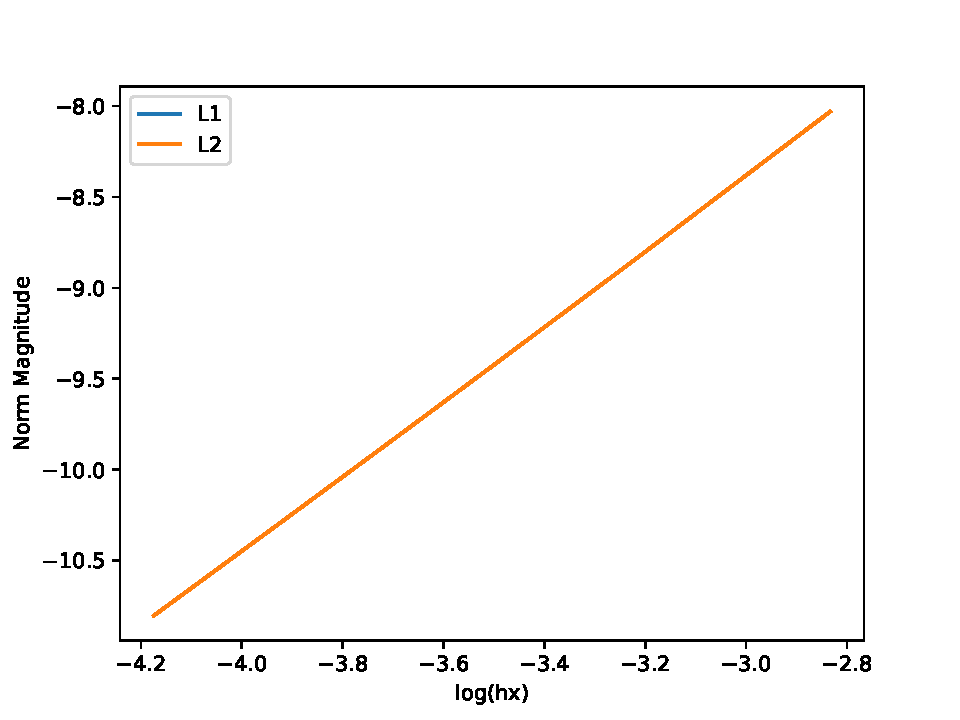
\includegraphics[width=0.8\textwidth]{temp_conv2.pdf}
	\caption{Convergence for benchmark 2}
\end{figure}

\begin{figure}
	\centering
	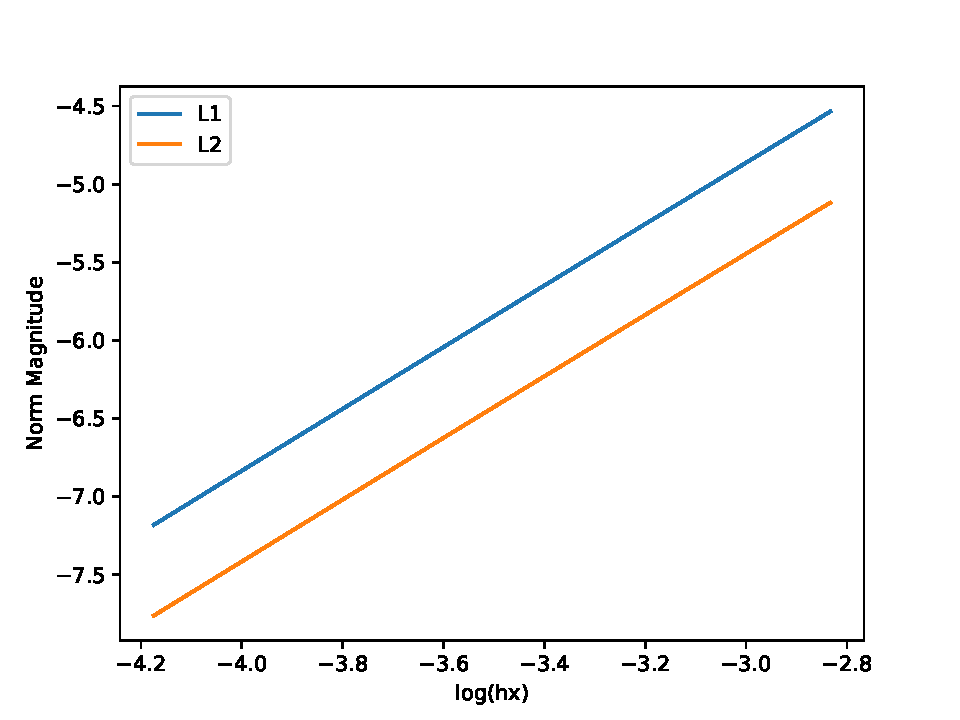
\includegraphics[width=0.8\textwidth]{temp_conv3.pdf}
	\caption{Convergence for benchmark 3}
\end{figure}